\section{Dataset Description}
\label{sec:data}

We study three public datasets that span qualitatively different network
types: a real-time social-media event, a corporate email archive, and a
friendship graph.
Table~\ref{tab:datasets} summarizes the key statistics of each network.

\begin{table}[ht]
\centering
\caption{Dataset statistics. Degree values are for the directed graphs
         (Higgs, Enron) or the undirected graph (Facebook).}
\label{tab:datasets}
\begin{tabular}{lrrrl}
\toprule
\textbf{Network} & \textbf{Nodes} & \textbf{Edges} & \textbf{Avg.\ Degree} & \textbf{Type} \\
\midrule
Higgs Mention  & 116{,}408 & 150{,}818 & 1.30 & Directed \\
Higgs Reply    &  38{,}918 &  32{,}523 & 0.84 & Directed \\
Higgs Retweet  & 256{,}491 & 328{,}132 & 1.28 & Directed \\
Enron Email    &  15{,}597 &  53{,}226 & 3.41 & Directed \\
Facebook       &   4{,}039 &  88{,}234 & 21.8 & Undirected \\
\bottomrule
\end{tabular}
\end{table}

\subsection{Higgs Twitter Dataset}

The Higgs Twitter dataset~\cite{higgs2013} was collected around July 4, 2012,
the day the discovery of the Higgs boson was announced.
It comprises three directed interaction networks derived from Twitter activity:

\begin{itemize}
    \item \textbf{Retweet network} (256{,}491 nodes): directed edge $(u \to v)$
          indicates that user $u$ retweeted a post by $v$.
          This is the largest and densest of the three networks.
    \item \textbf{Mention network} (116{,}408 nodes): directed edge $(u \to v)$
          indicates that user $u$ mentioned $v$ in a tweet.
    \item \textbf{Reply network} (38{,}918 nodes): directed edge $(u \to v)$
          indicates that user $u$ replied directly to a tweet by $v$.
          This is the smallest and most conversational of the three.
\end{itemize}

All three networks exhibit heavy-tailed in-degree distributions consistent
with a power-law, as shown in Figure~\ref{fig:higgs_deg}.

\begin{figure*}[ht]
    \centering
    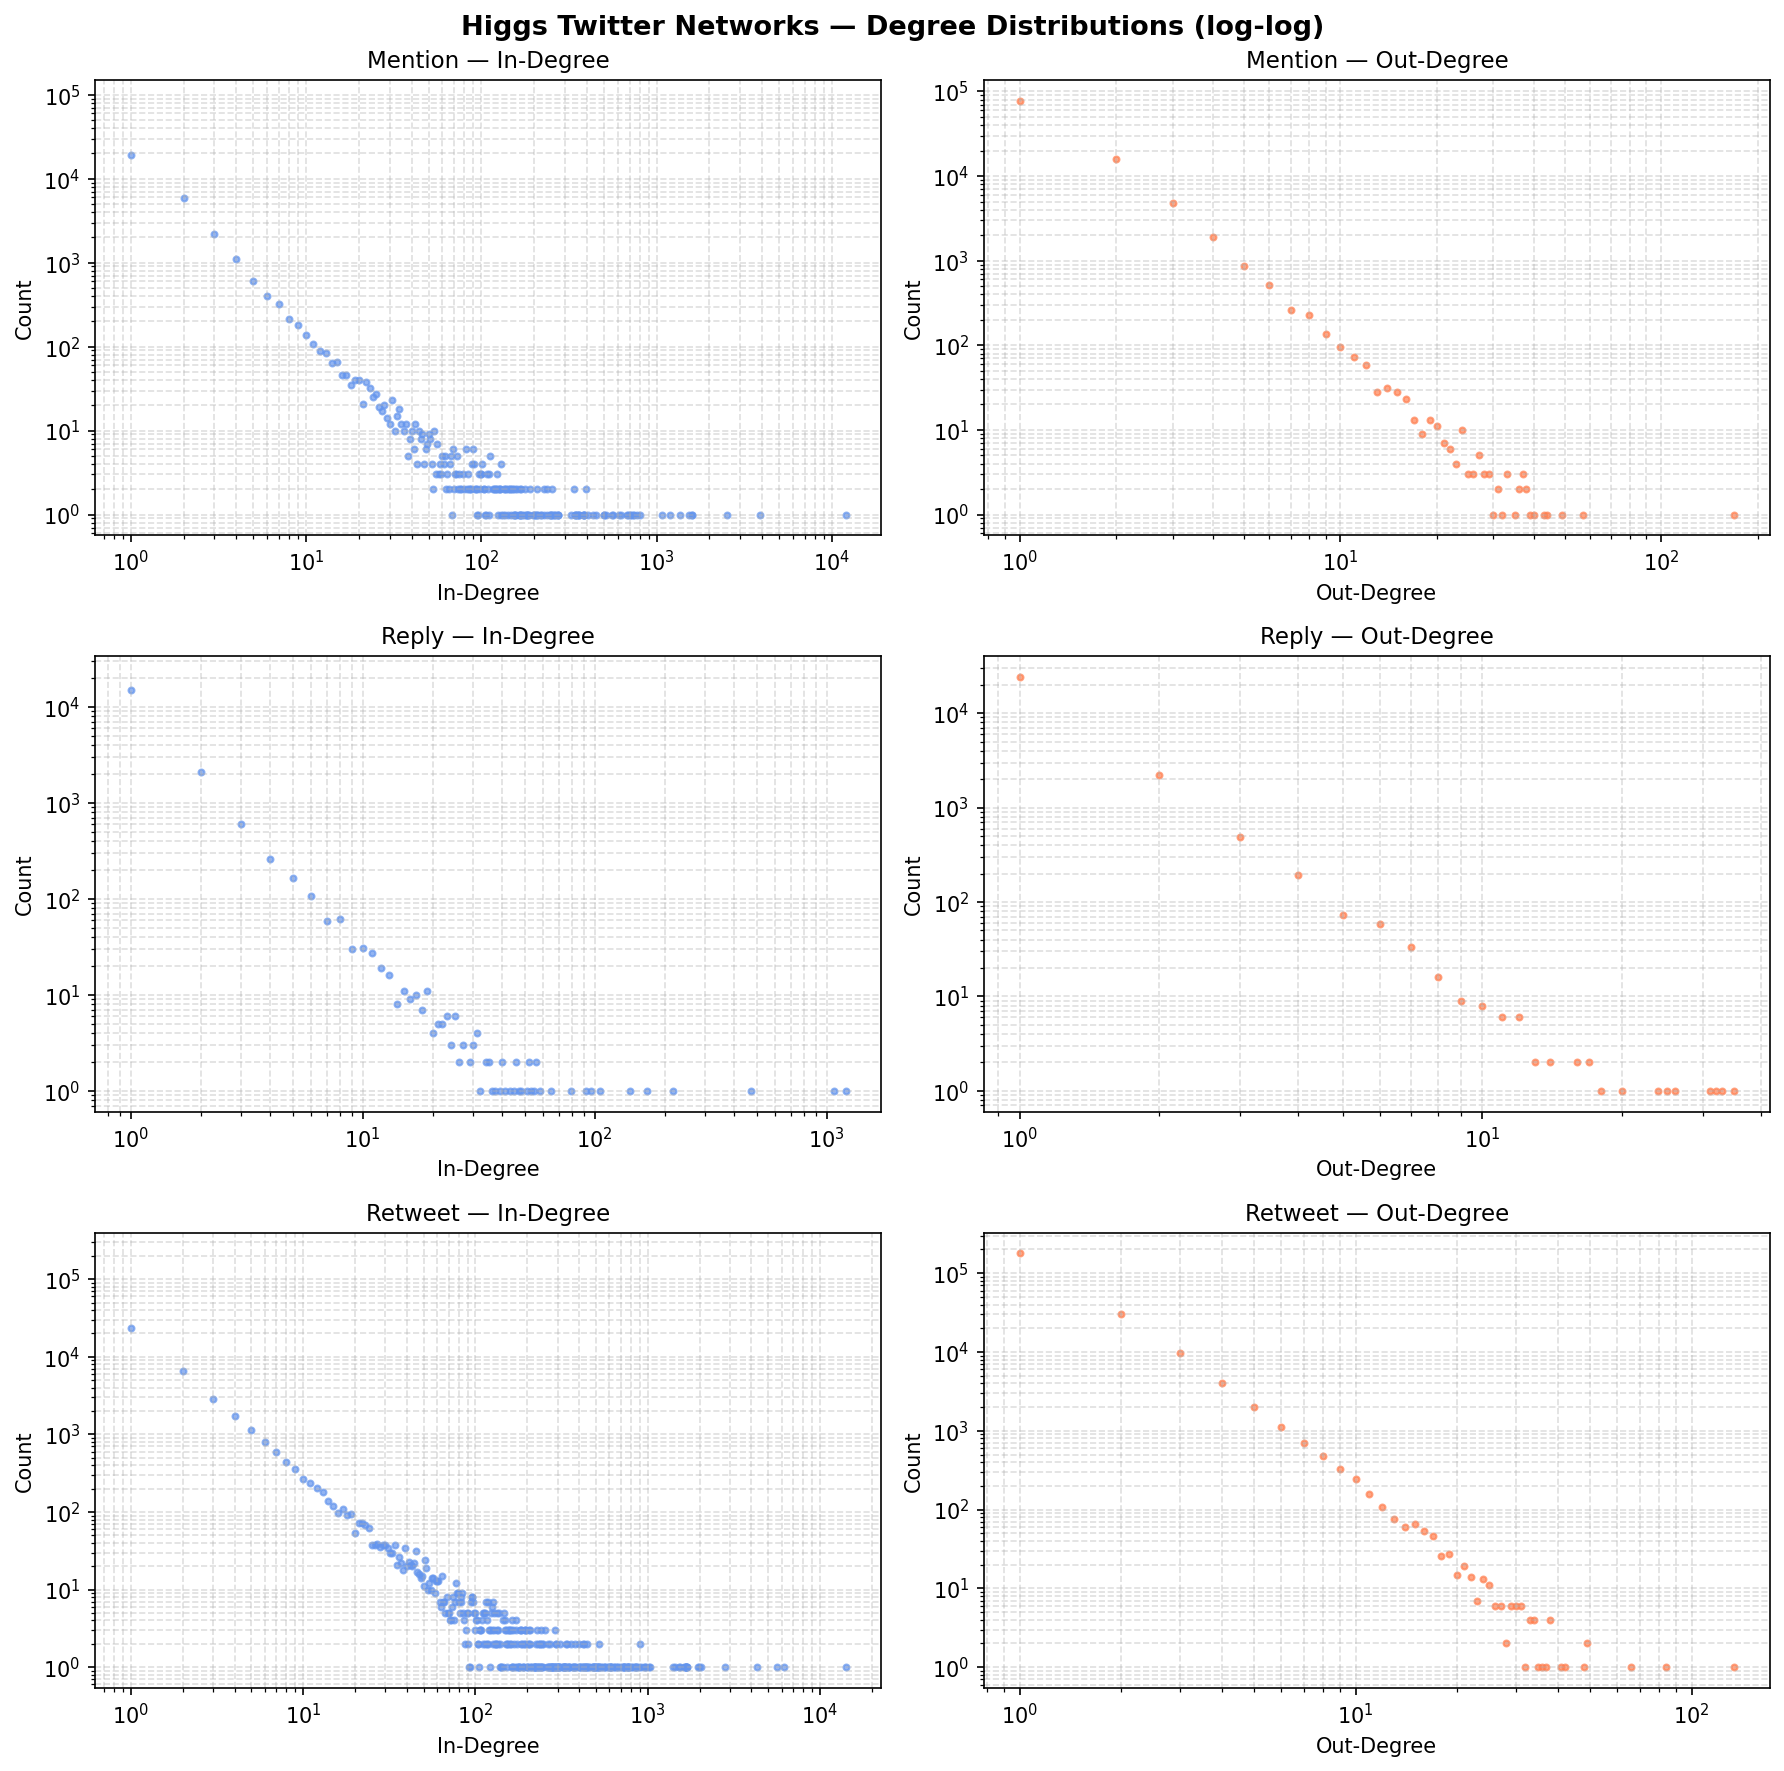
\includegraphics[width=0.85\linewidth]{figures/higgs_all_deg.png}
    \caption{Log-log degree distributions for the three Higgs Twitter networks
             (rows: Mention, Reply, Retweet), showing in-degree (left) and
             out-degree (right).
             All three exhibit heavy-tailed in-degree distributions consistent
             with preferential-attachment dynamics.
             Out-degree distributions are considerably more concentrated,
             indicating that most users participate moderately while a small
             number act as prolific broadcasters.}
    \label{fig:higgs_deg}
\end{figure*}

\subsection{Enron Email Dataset}

The Enron email dataset is derived from the publicly released Enron email
corpus and contains approximately 50{,}000 messages parsed for sender/receiver
pairs.
The resulting directed graph captures communication flow among
15{,}597 unique email addresses with 53{,}226 directed edges.
Figure~\ref{fig:enron_deg} shows the degree distribution of the
undirected projection.

\begin{figure}[!t]
    \centering
    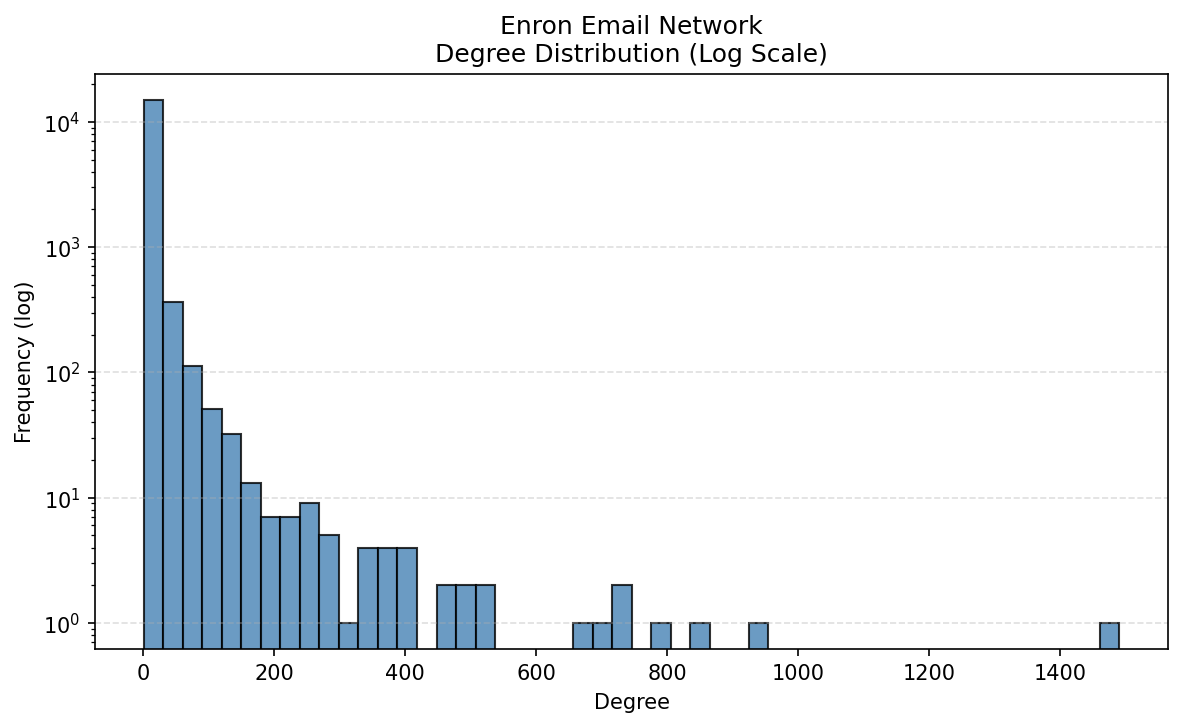
\includegraphics[width=0.9\linewidth]{figures/enron_deg.png}
    \caption{Degree distribution of the Enron email network (undirected
             projection, log scale).
             The distribution is heavy-tailed, with a small number of
             addresses — primarily executive inboxes and distribution lists —
             receiving a disproportionate volume of mail.}
    \label{fig:enron_deg}
\end{figure}

\subsection{Facebook Ego-Network Dataset}

The Facebook combined dataset~\cite{leskovec2012} comprises 4{,}039 nodes
and 88{,}234 undirected edges assembled from the ego-networks of ten
anonymized users.
With an average degree of 21.8, this is by far the densest of our three
datasets, reflecting the tightly clustered nature of real-world friendship
networks.
